%%%%%%%%%%%%%%%%%%%%%%%%%%%%%%%%%%%%%%%%%%%%%%%%%%
% Adam Newton Wright
% Appendix: LGS and Adaptive optics
% app.tex
%%%%%%%%%%%%%%%%%%%%%%%%%%%%%%%%%%%%%%%%%%%%%%%%%%

\appendix

%%%%%%%%%%%%%%%%%%%%%%%%%%%%%%%%%%%%%%%%%%%%%%%%%%
% Laser Guide Stars
%%%%%%%%%%%%%%%%%%%%%%%%%%%%%%%%%%%%%%%%%%%%%%%%%%
\chapter{Laser Guide Stars}

Telescopes observing distant astronomical objects face a significant challenge known as atmospheric distortion. Light coming from these astronomical objects travels in a straight line with little obstruction in the near vacuum of space. However, as a ray of light travels from free space into the atmosphere of Earth, it is affected by the many gaseous particles that make up the atmosphere and result in a different index of refraction than space. The effect is a bending of the light rays, known as \textit{refraction}, that can be described mathematically by Snell's Law, 

\begin{equation}
  n_1 \sin \theta_1 = n_2 \sin \theta_2,
  \label{snellslaw}
\end{equation}
%
where $n_1$ is the index of refraction of the first medium, $n_2$ is the refractive index of the second medium, and $\theta_1$ and $\theta_2$ are the angles that the ray makes with the normal to the interface between the media. A schematic of this is shown in Figure \ref{snellsfigure}.

\begin{figure}[ht!]
  \center
  \includestandalone{Images/tikz/snells}
\caption{Schematic of a ray of light refracting according to Snell's Law as it passes from a medium of refractive index $n_1$ into a medium with higher refractive index $n_2$.}
\label{snellsfigure}
\end{figure}

In general, the many light rays that make up the observed object will be refracted uniformly, causing the object to be perceived in a location that is different from its true position. While that alone is not a problem, if we look closer, we find that the atmosphere does not refract all light rays in the same manner, but small variations in pressure, temperature, and density cause a spatial variation in the index of refraction, resulting in light rays that are close together to be refracted in slightly different ways. This is known as \textit{atmospheric distortion}. A schematic is shown in Figure \ref{fig:atmosphericdistortion}, with plane waves being distorted as they pass through an atmosphere.


\begin{figure}[ht]
  \centering
  \includestandalone{Images/tikz/atmdistortion}
  \caption{Atmospheric distortion of a plane wave passing through Earth's atmosphere}
  \label{fig:atmosphericdistortion}
\end{figure}

The idea of atmospheric distortion will be familiar to those who have seen the sunset on the horizon. As the sun nears the horizon, the light is bent strongly through the atmosphere, resulting in much more distortion than when high in the sky. This results in a disfiguring of its spherical shape and a sharpening around the edges. An example of this is shown in Figure \ref{fig:sunset}.

\begin{figure}[t]
  \centering
  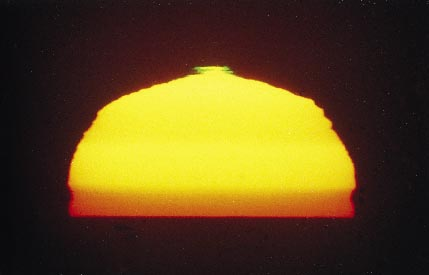
\includegraphics[width = .8\textwidth]{Images/sunset.jpg}
  \caption{Sunset with atmospheric distortion disfiguring the spherical shape of the sun and creating sharp patterns on the edges \protect\cite{sunset}.}
  \label{fig:sunset}
\end{figure}

In order for telescopes to improve resolution, astronomers need to find a way to rid their systems of this atmospheric distortion. One way to do this is to place the telescope outside of Earth's atmosphere where it would be unaffected by atmospheric distortion. This was done with amazing success in 1990 with the low-orbiting, powerful Hubble telescope \cite{Okolski}. However, it is not only extremely costly to put telescopes into orbit, but also impractical as they cannot be easily maintained or serviced.


Thus, a different solution was proposed. If astronomers could model how light was distorted as it passed through the atmosphere, they could subtract those distortions from their images and obtain higher resolution data. In order to measure the amount of distortion present, telescopes can observe a point source in the sky, such as a distant star, and observe its image. This image is then compared with the image of an ideal point source not affected by atmospheric distortion, and the difference between these two images represents the amount of distortion. Once the distortion is known, it is sent to a deformable mirror, which is made of many smaller mirrors, each able to move independently from the others. The deformable mirror can then create a wavefront conjugate to the distortion calculated. By reflecting the image of astronomical object off this mirror, the distortion is removed from the image. This process is known as \textit{adaptive optics}, and more information is given in Appendix B.


However, there are not always stars bright enough in the telescope's field of view that can be used as this point source (better known as a guide star) \cite{Wizinowich2006}. In order to skirt this problem, artificial stars were constructed, known as \textit{laser guide stars} (LGS). A laser guide star is created by sending laser light into the atmosphere, where it interacts with a layer of sodium atoms. These sodium atoms reside approximately $\SI{60}{\kilo\meter}$ from Earth in a $\SI{10}{\kilo\meter}$ thick layer of the atmosphere known as the mesosphere. A figure of this region within the layers of Earth's atmosphere is shown in Figure \ref{fig:mesosphere}. These atoms are deposited from meteors as they burn up in Earth's atmosphere, leaving behind their composite particles, a significant portion being sodium. The density of this sodium layer varies throughout a given day and throughout the year, but typically is near $\SI{5e13}{atoms \per \meter \cubed}$ \cite{Kibblewhite2009}. Using a laser with a wavelength resonant with sodium,  the atoms will absorb and emit this light, creating a glowing sphere in the upper atmosphere, as mentioned in Chapter 2. This sphere of light is then used as the guide star.\footnote{There are actually two types of laser guide stars: sodium based and Rayleigh scattering based. Rayleigh scattering laser guide stars rely on the scattering of light in the atmosphere, as opposed to having atoms absorb and emit light.}

\begin{figure}
		\center
		\includestandalone{Images/tikz/mesosphere}
	\caption{Schematic of sodium atoms residing in the mesosphere.}
	\label{fig:mesosphere}
\end{figure}



In general, most large-scale, ground-based telescopes now have powerful lasers with wavelengths precisely tuned to be resonant with sodium. As these telescopes are making observations, the lasers are shone into the sky to create the LGS. An image of an LGS being created is shown in Figure \ref{fig:LGSatESO}. The LGS is observed and atmospheric distortions are calculated and subtracted from the image in real time.

\begin{figure}[hb!]
  \centering
  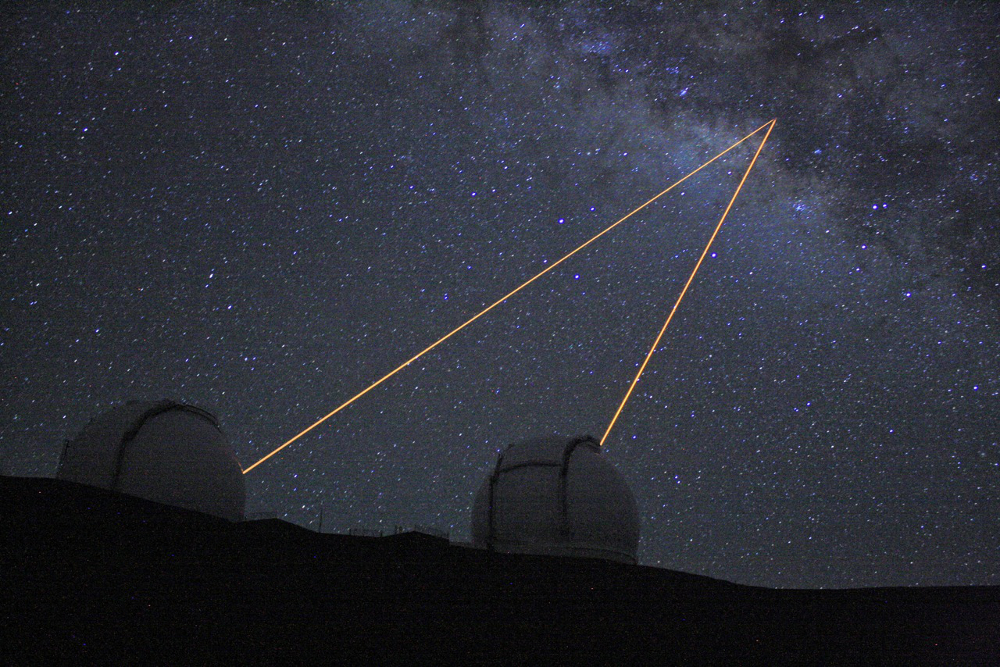
\includegraphics[width = .8\textwidth]{Images/LGSatESO.jpg}
  \caption{Laser guide star being created at the Very Large Telescope \protect\cite{VLT}.}
  \label{fig:LGSatESO}
\end{figure}

One major concern for LGS systems is their brightness in the sky \cite{Wizinowich2006}. It is important for the star to be bright enough that the telescope system is able to pick up enough light for a measurement of the distortion. The shape of the LGS is also important, as it must be as near to circular as possible in order for an accurate measurement of the distortion to be made. The shape of the LGS is mostly due to the profile of the laser beam \cite{Holzlohner2012} and will not be discussed here.

In order to create a brighter laser guide star, a few methods are utilized. One method is to increase the intensity, the power per unit area, of the laser. Typical laser intensities are of the order of \SI{20}{W \per \meter \squared} \cite{Kane2014}. This allows for more atoms to absorb and emit light, thereby creating a brighter star. Another method is to increase the diameter of the laser beam, which will allow for a greater area of sodium atoms to be reached by the light. These both have limitations, however. The power cannot continually be increased because of limitations on the power of lasers and due to downpumping \cite{Kane2014}. The size of the LGS also should not be continually increased since, for adaptive optics to work, the assumption is made that the LGS is a point source. A more sophisticated method, optical pumping (discussed in Chapter 2), makes use of circularly polarized light to move the atom into a cycling transition. The method explored in this thesis expounds on using circularly polarized light, but realizes the effects of the geomagnetic field on the distribution of angular momentum when circularly polarized light is used, and uses a pulsed laser to counteract this.


%%%%%%%%%%%%%%%%%%%%%%%%%%%%%%%%%%%%%%%%%%%%%%%%%%
% Adaptive Optics
%%%%%%%%%%%%%%%%%%%%%%%%%%%%%%%%%%%%%%%%%%%%%%%%%%

\chapter{Adaptive Optics}
The process of measuring the atmospheric distortion in order to enhance astronomical imaging, known as \textit{adaptive optics}, is a mathematical estimation problem. Here, we present an introduction to the methods used during this process.

In general, telescopes observe the LGS and the astronomical object simultaneously. The image of the LGS is then compared to an ideal point source imaged through the telescope without atmospheric distortion,\footnote{This is typically done using optical modelling software, but can also be done experimentally using various quasi-pointlike source objects.} and the distortion is calculated by comparing the two. A deformable mirror, composed of many smaller mirrors each of which can be moved independently of the others, is then used to create the opposite of the calculated distortion. The image of the astronomical object is then reflected off this mirror, thereby ridding the image of distortion.

In order to calculate the atmospheric distortion, astronomers make use of the well defined way in which point sources are imaged through optical systems. When an idealized point in object space is imaged through an optical system, it has a certain intensity distribution in image space, known as the point spread function. For an optical system with spherical symmetry and no aberration, the point spread function can be described mathematically along the radial coordinate $x$ as

\begin{equation}
	P(x) = \left(\frac{2 J_1(x)}{x}\right) ^{2},
  \label{psfa}
\end{equation}
%
where $P(x)$ is the intensity and $J_1(x)$ is the Bessel function of the first kind. This function is known as the \textit{Airy disk}, and is shown in Figure \ref{fig:airydiska}. It is an idealized description of a point imaged through a perfect optical system.

%\begin{figure}[h]
%  \centering
%  \begin{tikzpicture}
%	\begin{axis}
%	  \addplot3[surf,z buffer=sort,domain=-5:5,y domain=-5:5] gnuplot {airy((x**2+y**2)**(1/2))};
%	\end{axis}
%\end{tikzpicture}
%  \caption{<+caption text+>}
%  \label{fig:<+label+>}
%\end{figure}<++>




\begin{figure}[h]
  \centering
  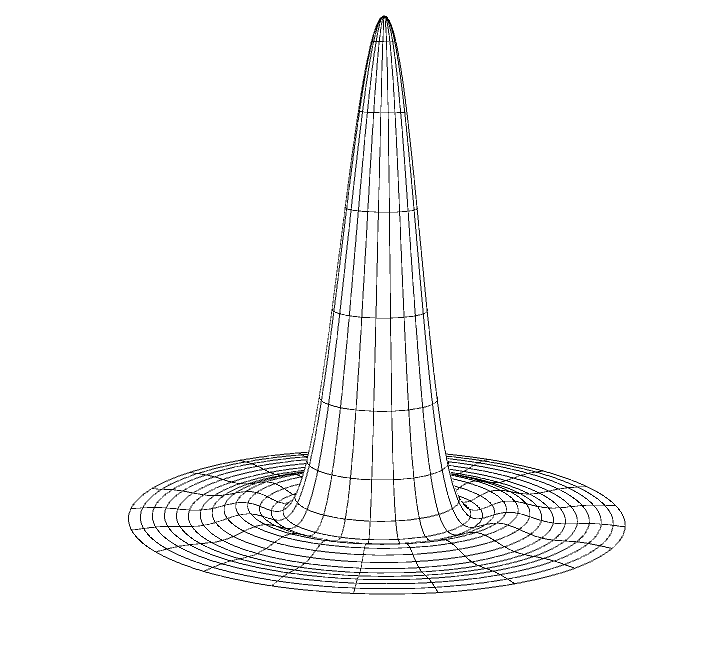
\includegraphics[scale = .4]{Images/airydisk.png}
  \caption{Graph of the Airy disk function where the height represents the intensity and the $x$ and $y$ axes represent spatial coordinates. The Airy disk describes an idealized point imaged through a spherically symmetric, aberration free optical system.}
  \label{fig:airydiska}
\end{figure}

It turns out that stars are very close to being point sources and can thus be used as this idealized point source. Since the light from these stars is passing through Earth's atmosphere, it will be distorted, and these distortions will show up in the point spread function, thus deviating from the Airy Disk described by Equation \ref{psfa}. 

Astronomers then use a combination of Fourier mathematics and an optimization algorithm to calculate the distortion. This method follows that outlined by Gonsalves \cite{Gonsalves1982}. This is done by first calculating optical transfer function

\begin{equation}
  H(\omega) = A(\omega) e^{i \theta(\omega)},
  \label{opticaltransfera}
\end{equation}
%
where $A(\omega)$ is the Fourier transform of the aperture function\footnote{The aperture function is a function describing where light can and cannot pass through. For a circular aperture, it would consist of a solid circle where light can pass through and nothing around the circle. It essentially acts like the computational version of a camera aperture.} of the system and $\theta(\omega)$ is the phase of the incoming light. The phase of the light can be described as a summation,

\begin{equation}
  \theta (\omega) = \sum _{k=0} ^{\infty} c_k \phi (\omega),
  \label{phasesuma}
\end{equation}
%
where $\{\phi (\omega) \}$ is a set of polynomials\footnote{The idea of using a set of polynomials to described the phase is similar to the idea of using sinusoidal functions in Fourier analysis to deconstruct a signal.} and $c_k$ is a coefficient that quantifies how much of each polynomial is present in the distortion. Taking the inverse Fourier transform and then the modulus squared, we can calculate the point spread function of this light

\begin{equation}
		P(x) = \Big|\text{ifft}[H(\omega)]\Big|^2,
  \label{otftopsfa}
\end{equation}
%
where $\text{ifft}$ denotes the inverse Fourier transform of the argument. This method allows us to mathematically create a point spread function simply by estimating the phase of the light with a set of polynomials.

Using this method, we have a way to estimate the distortion present in an image. First, a set of polynomials is selected. A possible set of polynomials to use is the Zernike set \cite{Gonsalves1982},\footnote{The Zernike set of polynomials can be used to described many optical distortions such as spherical aberration, defocus, coma, etc., and is chosen for systems displaying these distortions} but there are many others that can be used. Second, a coefficient list, or ``vector,'' of numbers is created in which each number will be the coefficient in front of its corresponding polynomial in the set of polynomials. This gives us a way to weight each of the polynomials in the set. Next, an algorithm is set up to change each number in the coefficient list, and, at each change, the point spread function is calculated (by the method above). This calculated, or estimated, point spread function is then compared to the observed point spread function, and an error metric is calculated. The algorithm will seek to minimize this error metric. Once this is minimized, the calculated point spread will be quite similar to the observed point spread function, and, at this point, we know the distortion acting on the system. The distortion is simply the set of polynomials, each weighted by its coefficient found by the algorithm.


Searching for the correct polynomials weighted by the correct coefficients is not trivial. Sometimes certain polynomials can be ignored if it is known by symmetry that they will not show up in the point spread function. Regardless, searching for the correct distortion is an optimization of a function in a large parameter space. Typical algorithms use a steepest descent approach \cite{Gonsalves1982}, which changes one parameter at a time, calculates an error between that estimation and the observed point spread function, and seeks to minimize this error. There have also been algorithms that use random searches, Monte Carlo walks, and Markov chain Monte Carlo searches that claim robustness and speed \cite{fienup}.

Once the correct distortion is calculated, the information is sent to the deformable mirror. This mirror consists of many smaller mirrors, each of which can be precisely adjusted by a piezoelectric actuator. The mirror changes shape, or adapts to the distortion,\footnote{This is where the term ``adaptive optics'' comes from.} creating a conjugate wavefront that the image from the telescope can be reflected off. At this point, the atmospheric distortion has been removed from the image. Normally, this is done in real time, and thus speed of both the calculation algorithm and of the movement of the deformable mirror must be optimized. Systems typically can calculate and adjust in under a second \cite{Wizinowich2006}.


%\begin{equation}
%  \begin{split}
%	Z_n^m (\rho,\phi) &= R_n^m (\rho) \cos(m\phi)\\
%	Z_n^{-m} (\rho, \phi) & = R_n^m (\rho) \sin(m\phi)\\
%	R_n^m (\rho) & = \sum _{k=0} ^{\frac{n-m}{2}} \frac{(-1)^k (n-k)!}{k!(\frac{n+m}{2}-k)! (\frac{n-m}{2}+k)}
%  \end{split}
%  \label{zernike}
%\end{equation}


%%%%%%%%%%%%%%%%%%%%%%%%%%%%%%%%%%%%%%%%%%%%%%%%%%
% Dye Lasers
%%%%%%%%%%%%%%%%%%%%%%%%%%%%%%%%%%%%%%%%%%%%%%%%%%

\chapter{Dye Lasers}
Dye lasers were some of the first lasers to be used as laser guide stars \cite{Primmerman1991}. This is due to a variety of factors: their wavelength can be precisely tuned over a broad spectral range, they are relatively inexpensive and easy to use,\footnote{Debatable once dye solution has spewed across half of the laboratory floor or fountained over the vacuum chamber. Also, some dyes cost 10 times more than gold per gram, likely invoking bitter feelings when one has to wipe up spilled liquid ``gold.'' Shout out to the LDS-798 backed currency though!} and they are fairly robust. However, recently many telescopes have opted for solid state or fiber lasers because of their efficiency and reliability \cite{Wizinowich2006}. My previous research dealt extensively with dye lasers, which is the main reason an MRP dye laser was first experimented with. Although it ultimately did not function as needed, we describe dye lasers in general, our proposed setup, and the problems that we encountered in this chapter.

\section{Introduction to Dye Lasers}
Laser is an acronym for \textit{light amplification by stimulated emission of radiation}. In general, a laser consists of three parts: a pump, a medium, and a cavity. The pump provides enough energy to move atoms in the medium into an excited state. The atoms then decay back into their ground state, releasing a photon in a random direction, which is known as spontaneous emission. However, a spontaneously emitted photon travelling through the medium can interact with another excited atom and stimulate the emission of a second photon through a process known as stimulated emission. This causes the excited atom to decay to its ground state, releasing a photon with the same direction, frequency, phase, and polarization as the initial photon. A cavity can be created around the medium, typically by placing mirrors on either side of the medium, causing the photons to travel back and forth in the medium, stimulating the emission of more and more photons. These photons will continue to build, creating a powerful source of monochromatic, coherent light. One of the cavity mirrors is commonly made partially transmissive, allowing only a certain percentage of photons to pass through and thus exit the cavity. These photons passing through the partially transmissive mirror form the usable laser beam. 

A dye laser, shown schematically in Fig. \ref{fig:dyelaser} works in exactly this way. Its medium is a fluorescent dye in a solvent such as methanol or ethanol. Typically, the pump is another laser with a wavelength of light corresponding to the absorption wavelength of the dye molecules. The cavity can vary in design but normally consists of a mirror at one end and a diffraction grating at the other. The diffraction grating spreads out the various wavelengths of light, allowing a specific wavelength to be diffracted back into the cavity through alignment of the grating. This results in a range of accessible wavelengths the system can lase at (tunability), typically on the order of a few tens of nanometers \cite{Sohl1997}. (More information of the basics of dye lasers and an easily constructable, undergraduate dye laser can be found in Sohl et al. \cite{Sohl1997}).

The big advantage of dye lasers is their incredible tunability over a broad spectral range. This is a consequence of the lasing medium. Since the fluorescence dye consists of large chain molecules, it can relax into one of its many vibrational and rotational states after being excited by the pump laser. This results in the molecule residing in a state that has slightly lower energy than the excited state. Thus, photons emitted from these states will have varying wavelengths, typically tens of nanometers longer than the absorption wavelength. In order to access and select these different wavelengths, the diffraction grating is used to split apart the various wavelengths, sending the desired lasing wavelength back into the medium. This specific wavelength then stimulates the emission of photons of similar wavelength, narrowing the linewidth of the laser light.

\begin{figure}[ht]
%	\centering
	\includestandalone{Images/tikz/dyelaser}
  \caption{Schematic of a dye laser. The medium, a fluorescent dye solution in the dye cell, is excited by a laser pump beam and lasing in a cavity consisting of a mirror and diffraction grating. The $0^{th}$ order diffracted beam forms the output laser beam while the $1^{st}$ order diffracted beam is reflected back into the cavity.}
  \label{fig:dyelaser}
\end{figure}


An ultrashort pulsed dye laser, with pulse widths on the order of picoseconds and repetition rates of hundreds of kilohertz (a pulse period on the order of \SI{1}{\micro \second}) is significantly more difficult to construct than a CW or long-pulse dye laser. In order to create a significant amount of stimulated emission, photons must have enough time to travel back and forth through the cavity a number of times\footnote{Technically, only one pass through the cavity is sufficient, but increasing to around 10 passes allows for a significant narrowing of the linewidth.} to induce the stimulated emission of more photons from molecules in an excited state. For ultrashort pulses, there are only a few picoseconds of time for the light to interact with the molecules per pulse. Once the pulse has excited the molecules, there is then a certain timescale (lifetime) over which the atoms will stay excited. The dye we use (Rhodamine 6G) has a lifetime of a few nanoseconds \cite{Selanger1977}. Thus, each molecule sees only a single laser pulse, which is why the lifetime will determine the timescale. The pulse widths and lifetime of the dye are shown in Fig. \ref{fig:tikzpulses}. This is different than a laser with a pulse width on the order of \SI{1}{\nano \second}, where the lifetime is much shorter than the pulse width. For a longer pulse width laser, the pulse width of the laser would determine the timescale.

In order to construct this dye laser cavity, we need to determine the necessary length of the cavity. A shorter cavity will allow for photons to complete more round trips creating more laser light. In the time that the dye is excited, photons should complete around ten trips through the cavity. The length of the cavity must then be on the order of, or shorter than,

\begin{equation}
  \begin{split}
  L & = \frac{1}{10} c \tau  \approx \SI{0.03}{\meter},\\
\end{split}
  \label{cavitylength}
\end{equation}
%
where $L$ is the total length of the lasing cavity, $c$ is the speed of light, and $\tau$ is lifetime of the dye. Experimentally, $\SI{3}{\centi\meter}$ is a tight fit for a laboratory-built cavity. Furthermore, because of the short interaction time between the pulse and the molecules, it is possible not enough molecules are being excited per laser pulse. Thus, constructing and aligning this laser proves difficult.

\begin{figure}[htpb]
	\centering
	\includestandalone[width=0.9\textwidth]{Images/tikz/pulses}
	\caption{Pulses of the pump laser shown in solid lines, with pulse width on the order of \SI{1}{\pico \second} and period on the order of \SI{1}{\micro \second}. The dashed lines indicate the lifetime of the dye, which is on the order of \SI{1}{\nano \second}.}
	\label{fig:tikzpulses}
\end{figure}



%%%%%%%%%%%%%%%%%%%%%%%%%%%%%%%%%%%%%%%%%%%%%%%%%%
% Second Harmonic Generation
%%%%%%%%%%%%%%%%%%%%%%%%%%%%%%%%%%%%%%%%%%%%%%%%%%

\section{Second Harmonic Generation}

An important part of a dye laser is the pump source that excites the medium. A common way to pump a dye laser is with another laser of wavelength equal to the absorption wavelength of the dye. The dye we use has an absorption wavelength around \SI{532}{\nano \meter}. However, the pump laser we have, while capable of a repetition rate equal to the Larmor frequency, lases in the infrared at $\lambda = \SI{1064}{\nano \meter}$. Thus, we need to convert $\SI{1064}{\nano \meter}$ light into light near \SI{532}{\nano \meter}.\footnote{The dye molecules, being relatively large, can absorb at many wavelengths and thus do not need a specific and precise wavelength for absorption to occur.} This can be done using a frequency doubling crystal, which converts photons of $\SI{1064}{\nano \meter}$ into photons of $\SI{532}{\nano \meter}$. This is known as second harmonic generation and is outlined in this section.

The electric field of an electromagnetic wave can be described by

\begin{equation}
  E_i = \varepsilon _i e^{-i\omega t},
  \label{harmonicfield}
\end{equation}
%
where $\varepsilon_i$ is the amplitude of the field at the given location, $\omega$ is the frequency, and $t$ is time \cite{Dood2006}. For a linear crystal, the polarization created in the crystal by the electric field can be described by a linear function

\begin{equation}
  \vec P = \epsilon _0 \chi^{(1)} \vec E,
  \label{linearpolarization}
\end{equation}
%
where $\epsilon_0$ is the permittivity of free space, $\chi^{(1)}$ is the linear electric susceptibility,\footnote{The linear electric susceptibility is a constant that relates polarization inside a medium to the induced electric field. It is given by $\chi = \epsilon_r - 1$ where $\epsilon_r$ is the dielectric constant. Thus, in a vacuum where $\epsilon_r = 1$, we can see that $\chi = 0$. In more complex media, such as anistropic crystals, the susceptibility becomes a tensor.} and $\vec E$ is the external electric field. The polarization is thus the electric field multiplied by a constant.

However, nonlinear crystals behave much differently than linear crystals due to their unique, atypical polarization. These crystals create a nonlinear polarization function which can be written (using the Taylor expansion) as

\begin{equation}
  \vec P = \epsilon _0 \left( \chi^{(1)}_{ik}E^i + \chi^{(2)}_{ijk} E^i E^j + \chi^{(3)}_{ijlk}E^i E^j E^l +\dots \right),
  \label{nonlinearpolarization}
\end{equation}
%
where each $\chi^{(n)}$ represents the tensor of the $n^{th}$ order susceptibility and the notation $\chi_{ik} E_i$ corresponds to an Einstein summation.\footnote{Einstein notation is a shorthand way of writing summations. For any repeated index that appears in a subscript and superscript, we compute a summation over that index. For example, $\chi _{ik}E^i = \sum_{i=1} \chi_{ik}E_i$.} If we now substitute in the electric field from Eq. \ref{harmonicfield}, we see that we will get terms of order $E^2$. If we look specifically at the polarization for these second order terms, we find that the polarization is

\begin{equation}
  P_k = \epsilon_0 \left( \varepsilon_j \varepsilon_k e^{-2i\omega t} + \varepsilon_j^* \varepsilon_k^* e^{2i\omega t} + \varepsilon_j^* \varepsilon_k + \varepsilon_j \varepsilon_k^* \right),
  \label{freqdoubledfield}
\end{equation}
%
where the superscript $^*$ denotes complex conjugate and $j,k \in \{ x,y,z \}$ are indices. Thus, we find terms of $e^{2i\omega t}$, implying that not only do we have the linear field with frequency $\omega$, but we have picked up a field with frequency $2\omega$ \cite{Dood2006}. In the crystals we will be using, the second-order term will dominate when the laser intensity is high, implying a majority of light is frequency doubled by the nonlinear term and a negligible amount of light passes through without being doubled.


This is second harmonic generation and is a process that occurs in nonlinear crystals where two photons of frequency $f_1$ are converted into one photon of frequency $f_2$ with $2 f_1 =f_2$. Since the energy of a photon is linearly proportional to its frequency, this makes intuitive sense from a conservation of energy perspective. A depiction of this is shown in Fig. \ref{fig:SHG}, where the initial light is known as the fundamental wave and frequency doubled light is known as the second harmonic wave.

%\begin{figure}[ht!]
%  \centering
%  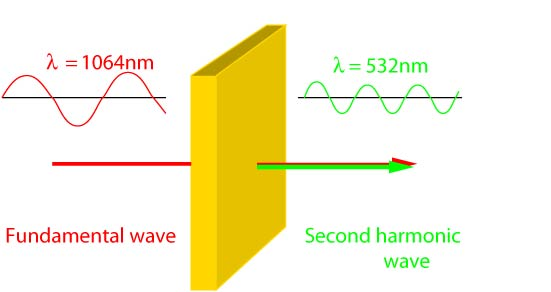
\includegraphics[width = .8\textwidth]{Images/SHG.jpeg}
%  \caption{Depiction of second harmonic generation where an incoming photon, travelling through a nonlinear crystal (yellow block), is converted into two photons, each with half the frequency as the initial photon \protect\cite{SHG}.}
%  \label{fig:SHG}
%\end{figure}

\begin{figure}[ht!]
  \centering
  \includestandalone[width = .8\textwidth]{Images/tikz/shg}
  \caption{Depiction of second harmonic generation where two incoming photons of frequency $f_1$, travelling through a nonlinear crystal, are converted into one photon with frequency $f_2 = 2f_1$, with some light of frequency $f_1$ left over \protect\cite{SHG}.}
  \label{fig:SHG}
\end{figure}
%Birefringence is the property of a material having different refractive indices based upon the polarization of the incoming light; this is unique since for most materials, the index of refraction is uniform and dependent only upon the wavelength of light. For birefringent materials, their exists two different indices of refraction; each of these indices occur when the polarization is parallel to a specific axis within the crystal. These two axes are known as the \textit{ordinary} axis and the \textit{extraordinary} axis; light with polarization along the ordinary axis will follow the standard rules of refraction (hence the name ordinary), given by Equation \ref{snellslaw}. However, light with polarization along the extraordinary axis will travel at a speed different from the light with ordinary polarization due to the difference in the index of refraction the light ``sees'' along each of these axes.

In order to achieve maximum efficiency during a frequency doubling conversion, the phase difference between the fundamental and second harmonic needs to be approximately zero, ensuring that no destructive interference occurs. The necessary condition is shown in Fig. \ref{fig:phasematching}, with the wave-vector $\vec{k}$ of the fundamental and second harmonic wave shown. The wave-vector is a vector of magnitude equal to the wavenumber (inverse wavelength) of the wave and direction equal to its propagation direction.



\begin{figure}[h]
  \centering
  \includestandalone{Images/tikz/phasematching}
  \caption{Shown is the phase matching condition of the fundamental and second harmonic wave. In order to achieve maximum efficiency, $\Delta \vec k \approx 0$.}
  \label{fig:phasematching}
\end{figure}

Mathematically, we can define the difference $\Delta \vec k$ between the waves as the sum of the fundamental wave-vector plus twice the second harmonic wave-vector. This relation is

\begin{equation}
  \Delta \vec k = \vec k_1 - 2 \vec k_2,
  \label{phasematching}
\end{equation}
%
where $\vec k_1$ is the wavenumber of the fundamental wave, and $\vec k_2$ is the wavenumber of the second harmonic. Having a difference of $\Delta \vec k = 0$ ensures that no destructive interference between the waves will occur, resulting in maximum output power.

\section{Characteristics of the Dye Laser}

The dye laser consisted of a quartz cell filled with fluorescent rhodamine-6G dye dissolved in methanol and a mirror-diffraction grating cavity and was pumped by a Nd:YVO$_4$ solid state laser.

%%%%%%%%%%%%%%%%%%%%%%%%%%%%%%%%%%%%%%%%%%%%%%%%%%
% dyes
%%%%%%%%%%%%%%%%%%%%%%%%%%%%%%%%%%%%%%%%%%%%%%%%%%
When constructing the laser, we used rhodamine-6G as a dye primarily because of its low cost. The rhodamine 6G was dissolved in methanol at an ideal concentration of \SI{0.10}{\gram \per \liter}. Rhodamine 6G, however, does not lase at the wavelength needed for rubidium but instead lases around \SI{566}{\nano \meter}. Once the laser was constructed, we intended to switch to LDS-798, which lases around \SI{785}{\nano \meter}. More information about lasing wavelength, solvents, efficiencies, and concentrations can be found in \textit{Lambdachrome Laser Dyes} \cite{Brackmann2000}.

The dye laser was pumped by a frequency doubled Nd:YVO$_4$ laser with a variable repetition rate from \SI{200}{ kHz} to \SI{4}{ MHz}, a pulse width of \SI{10}{\pico \second}, and wavelength of \SI{1064}{\nano \meter}. The laser produced an average power of around \SI{13}{W} at \SI{200}{\kilo Hz}. The dye solution  absorbs in the visible range, not the infrared, which created the necessity for frequency doubling.

When using a frequency doubling crystal, it is important to maintain the alignment and temperature of the crystal, since both of these can impact the performance of the second harmonic generation process. The temperature of the crystal was controlled using a transistor-thermistor combination. The transistor controlled whether current flowed through the crystal housing. If current did flow, the transistor would heat up, in turn heating up the crystal. The temperature of the crystal was monitored using a thermistor, a resistor whose resistance changes with temperature. 

In order to accurately monitor the temperature, the thermistor needs to be calibrated. This was done by allowing current to pass through the transistor and measuring the resistance of the thermistor at various temperatures (measured with a mercury thermometer). The data used for this calibration are shown in Fig. \ref{fig:rvt}. It was found that the temperature followed the function

\begin{equation}
	T = (-0.21 \pm 0.01)  R + (117.74 \pm 1.28),
	\label{eq:RvT}
\end{equation}
%
where $R$ is the resistance in Ohms and $T$ is the temperature in degrees Celsius. This allowed the temperature of the crystal to be measured by simply measuring the resistance of the thermistor.


%%%%%%%%%%%%%%%%%%%%%%%%%%%%%%%%%%%%%%%%%%%%%%%%%%
% Figure of temperature versus resistance for thermistor
%%%%%%%%%%%%%%%%%%%%%%%%%%%%%%%%%%%%%%%%%%%%%%%%%%
\begin{figure}[h]
  \centering
  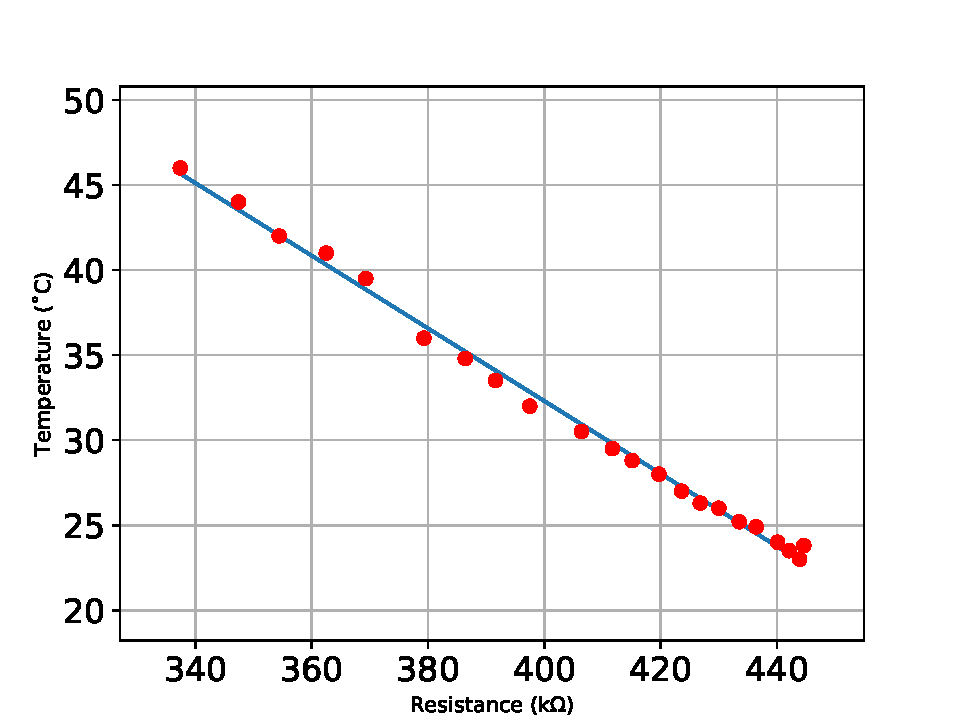
\includegraphics[width = .8\textwidth]{Images/bestfitRvT.pdf}
  \caption{Temperature of the thermistor as a function of its resistance. A linear best fit function is plotted, given by Eq. \ref{eq:RvT}.}
  \label{fig:rvt}
\end{figure}


The temperature of the crystal was also measured as a function of the current through the transistor. A specific current was supplied to the transistor, two minutes were allotted for the crystal to heat up, and the temperature was then measured with a mercury thermometer. A figure of these data is shown in Fig. \ref{fig:tvsi}, and the temperature is shown to increase rapidly as current increases.

%%%%%%%%%%%%%%%%%%%%%%%%%%%%%%%%%%%%%%%%%%%%%%%%%%
% Temperature versus current
%%%%%%%%%%%%%%%%%%%%%%%%%%%%%%%%%%%%%%%%%%%%%%%%%%
\begin{figure}[h!]
  \centering
  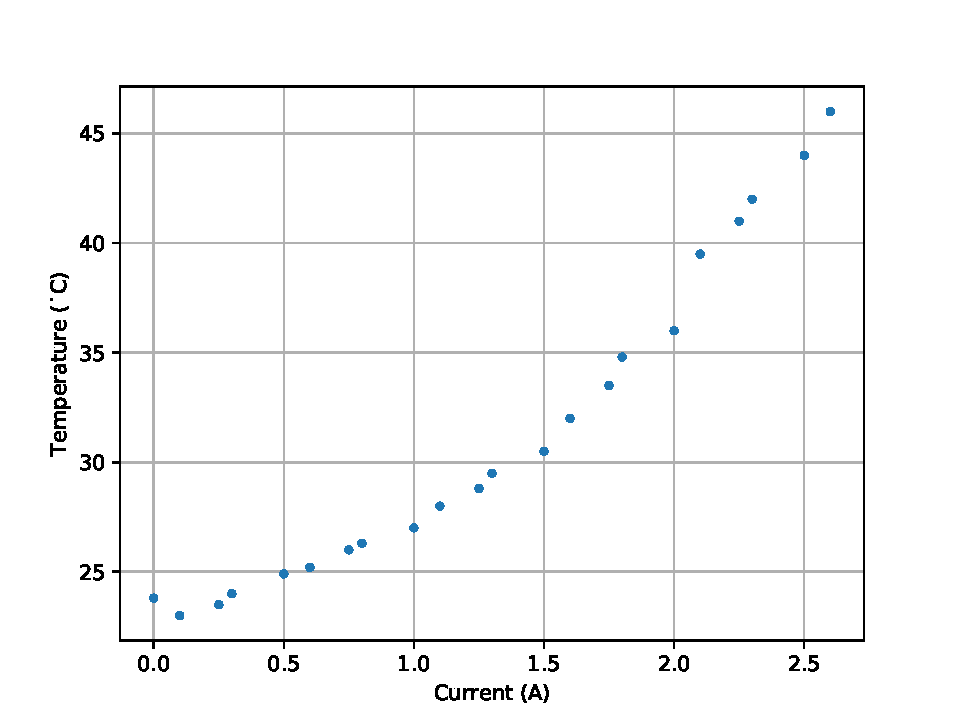
\includegraphics[width = .8\textwidth]{Images/TvsI.pdf}
  \caption{Graph of the temperature of the crystal plotted versus current through the transistor.}
  \label{fig:tvsi}
\end{figure}


Two times series were also taken of the resistance of the thermistor and the temperature of the crystal. These were both measured by running \SI{5}{ A} of current through the transistor. The resistance decreases rapidly over time with very small fluctuations in resistance, as shown in Fig. \ref{fig:resfluct}. The temperature increases exponentially in time with small fluctuations, especially at higher temperatures. These fluctuations, however, may simply be an artifact of the thermometer as opposed to actual temperature fluctuations in the crystal. The temperature versus time data are shown in Fig. \ref{fig:tempflucfit}, along with an exponential best fit for the temperature data, given by

\begin{equation}
	T = 47.7 - 22.7 e^{-t/308.7},
	\label{eq:temptime}
\end{equation}
%
where $T$ is the temperature in degrees Celsius and $t$ is time in seconds.


%%%%%%%%%%%%%%%%%%%%%%%%%%%%%%%%%%%%%%%%%%%%%%%%%%
% Resistance versus times
%%%%%%%%%%%%%%%%%%%%%%%%%%%%%%%%%%%%%%%%%%%%%%%%%%
\begin{figure}[h!]
  \centering
  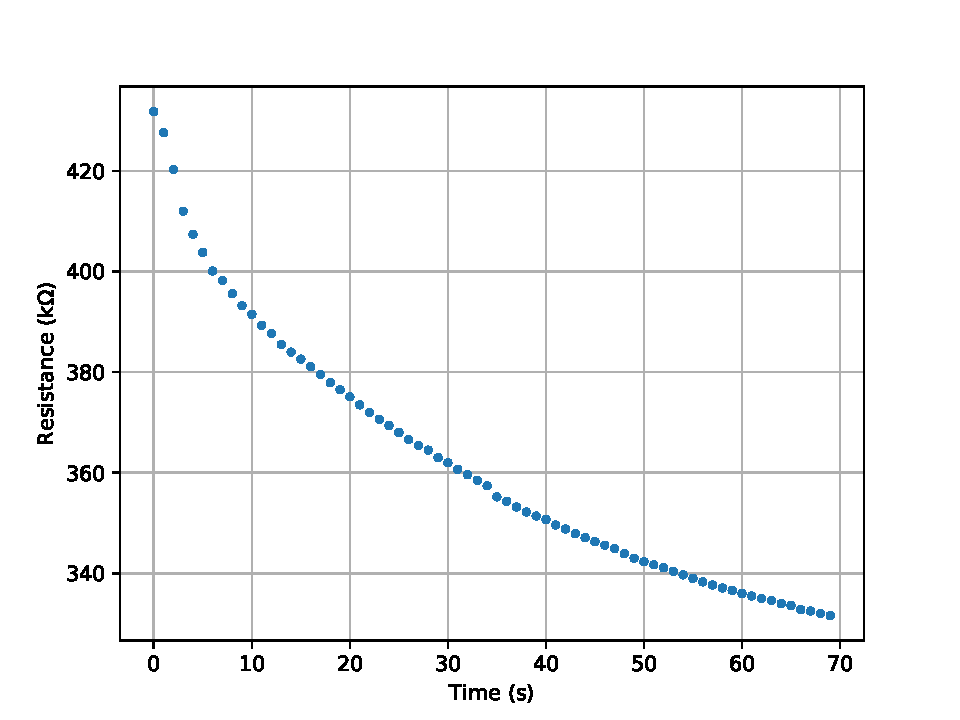
\includegraphics[width = .8\textwidth]{Images/ResFluct.pdf}
  \caption{Graph of the change in resistance of the thermistor over time at fixed current of \SI{5}{ A}.}
  \label{fig:resfluct}
\end{figure}
%%%%%%%%%%%%%%%%%%%%%%%%%%%%%%%%%%%%%%%%%%%%%%%%%%
% Temperature versus time
%%%%%%%%%%%%%%%%%%%%%%%%%%%%%%%%%%%%%%%%%%%%%%%%%%
\begin{figure}[h!]
  \centering
  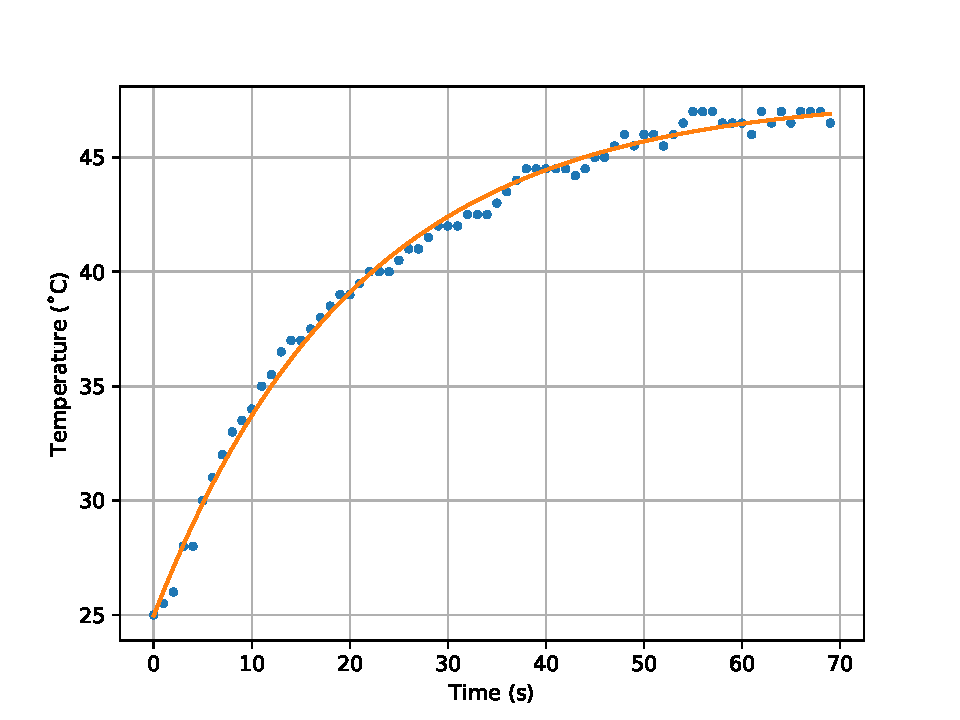
\includegraphics[width = .8\textwidth]{Images/TempFluctFit.pdf}
  \caption{Graph of the change in temperature as a function of time at fixed current of \SI{5}{ A}. An exponential best fit is plotted on top of these data, given by Eq. \ref{eq:temptime}.}
  \label{fig:tempflucfit}
\end{figure}

The crystal, transistor, and thermistor were found to function according to expectations, and were thus ready to be used for second harmonic generation. Using a spectrometer to measure the wavelength of light transmitted through the crystal, the crystal was aligned for optimal conversion of \SI{1064}{\nano \meter} light into \SI{532}{\nano \meter} light. This was done with \SI{5}{ A} of current running through the transistor in order to heat the crystal. A figure of the spectrum at poor alignment is shown in the left panel of Fig. \ref{fig:conversionspectrum1}, where the peak on the left is the amount of \SI{532}{\nano \meter} light transmitted and the peak on the right is the amount of \SI{1064}{\nano \meter} light transmitted through the crystal. It can be seen that only a small fraction of the fundamental light is converted into the second harmonic light. The crystal was most sensitive to rotations about the axis perpendicular to the optical axis, but its efficiency depended also upon vertical and horizontal adjustments. At optimal alignment, the crystal converted roughly 65\% of the initial \SI{1064}{\nano \meter} light into \SI{532}{\nano \meter} light. This can be seen in the right panel of Fig. \ref{fig:conversionspectrum1}, where more \SI{532}{\nano \meter} light is seen than \SI{1062}{\nano \meter} light. Typically, conversion efficiencies (amount of \SI{532}{\nano \meter} light divided by the amount of \SI{532}{\nano \meter} plus \SI{1064}{\nano \meter} light) above 50\% are expected and around 70\% to 80\% are good. For our purposes, 65\% was sufficient to excite the dye solution to be used in the dye laser.

%%%%%%%%%%%%%%%%%%%%%%%%%%%%%%%%%%%%%%%%%%%%%%%%%%
% Figure of spectrum of crystal
%%%%%%%%%%%%%%%%%%%%%%%%%%%%%%%%%%%%%%%%%%%%%%%%%%
\begin{figure}[h!]
  \centering
  \begin{minipage}{.45\textwidth}
	  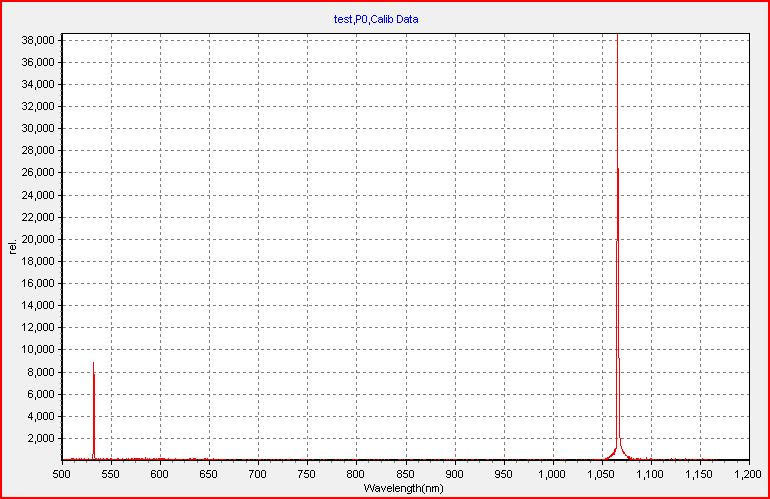
\includegraphics[scale = .32]{Images/doublingCrystalWright2017.JPG}
  \end{minipage}
  \begin{minipage}{.45\textwidth}
	  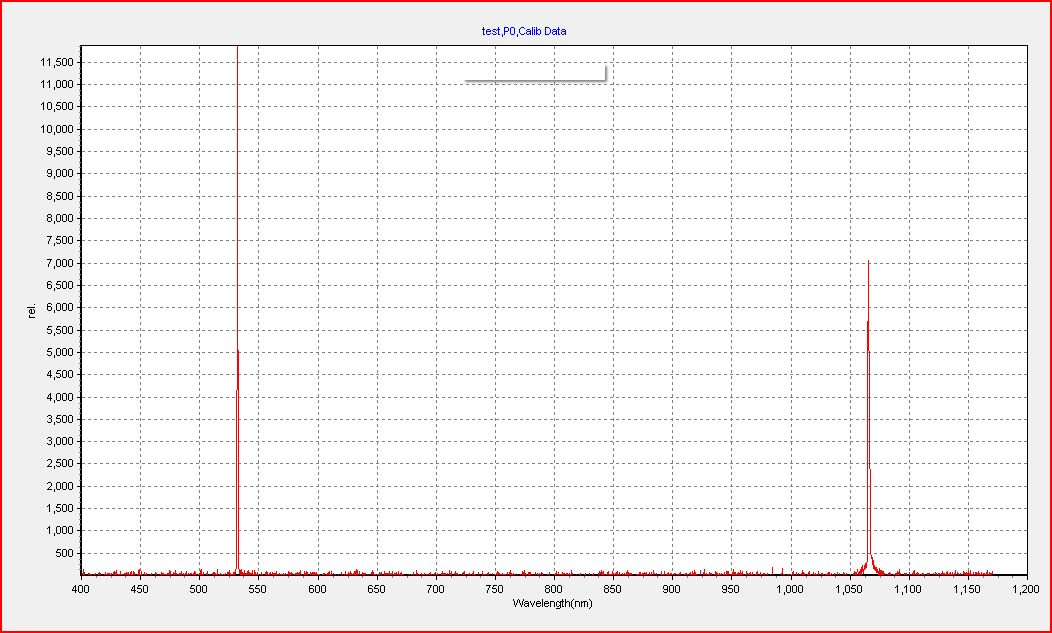
\includegraphics[scale = .25]{Images/goodspectrum.JPG}
  \end{minipage}
  \caption{Spectra of converted laser light through doubling crystal before alignment (left) and after alignment (right). \SI{532}{\nano \meter} light shown on the left peak and \SI{1064}{\nano \meter} light shown on the right peak.}
  \label{fig:conversionspectrum1}
\end{figure}

With spatial alignment optimized, the conversion efficiency also needed to be optimized with respect to the temperature of the crystal. In optimal spatial alignment, at maximum temperature (current at \SI{5}{ A}), the current was turned off and the conversion efficiency was measured at various resistances. Since resistance depends upon temperature, this gives a measurement of efficiency versus temperature. These data are shown in Fig. \ref{fig:crystaleff}, and the efficiency clearly decreases with increasing resistance. Since temperature decreases with increasing resistance, it was decided that in order to convert the maximum amount of \SI{532}{\nano \meter} light, the temperature needed to be increased. However, even with temperatures above the previously mentioned test, the conversion efficiency never exceeded the previously measured 65\%. This efficiency turned out to be the maximum conversion efficiency. Any deviations from it were simply misalignments as the temperature changed. For all temperatures, the 65\% efficiency could be established through spatial re-alignment. Thus, since the conversion efficiency was not dependent upon the temperature of the crystal but only upon spatial alignment, we did not stabilize the temperature of the crystal.

With the medium and pump of the dye laser constructed, the cavity needed to be constructed and aligned. The final cavity would consist of a silver coated mirror on one end and a diffraction grating on the other, schematically shown in Fig. \ref{fig:dyelaser}. However, for initial alignment, it is easiest to replace the diffraction grating with a glass slide acting as a partially transmissive mirror. The cavity was initially aligned by pumping the medium with a \SI{532}{\nano \meter} Nd:YAG solid state laser, with a repetition rate of \SI{10}{ Hz} and a pulse width on the order of \SI{10}{\nano \second}. This made initial alignments much easier due to the longer pulse width of the Nd:YAG laser. After the cavity was lasing through excitation with the Nd:YAG laser, the Nd:YAG was turned off and the Nd:YVO$_4$ was switched on. The cavity was then realigned through excitation in an attempt to ellicit lasing from the Nd:YVO$_4$. However, no lasing was ever seen. Power meters, photodiodes, and spectrometers were employed to search for small amounts of lasing light from the cavity but yielded no results. It was concluded that the pulse width of the pump beam was indeed too short for our cavity to lase, and the dye laser was abandoned.

It should be noted that a superposition of lasers beams was also attempted. It was thought that small amounts of stimulated emission could be produced with the longer pulse Nd:YAG, and then, by overlapping the Nd:YVO$_4$ beam with the Nd:YAG beam, the dye laser could be pushed over the threshold and begin lasing. There are various problems with this (e.g. beating), but regardless, lasing was still not established.

%%%%%%%%%%%%%%%%%%%%%%%%%%%%%%%%%%%%%%%%%%%%%%%%%%
% Figure of the efficiency of the crystal
%%%%%%%%%%%%%%%%%%%%%%%%%%%%%%%%%%%%%%%%%%%%%%%%%%
\begin{figure}[h!]
  \centering
  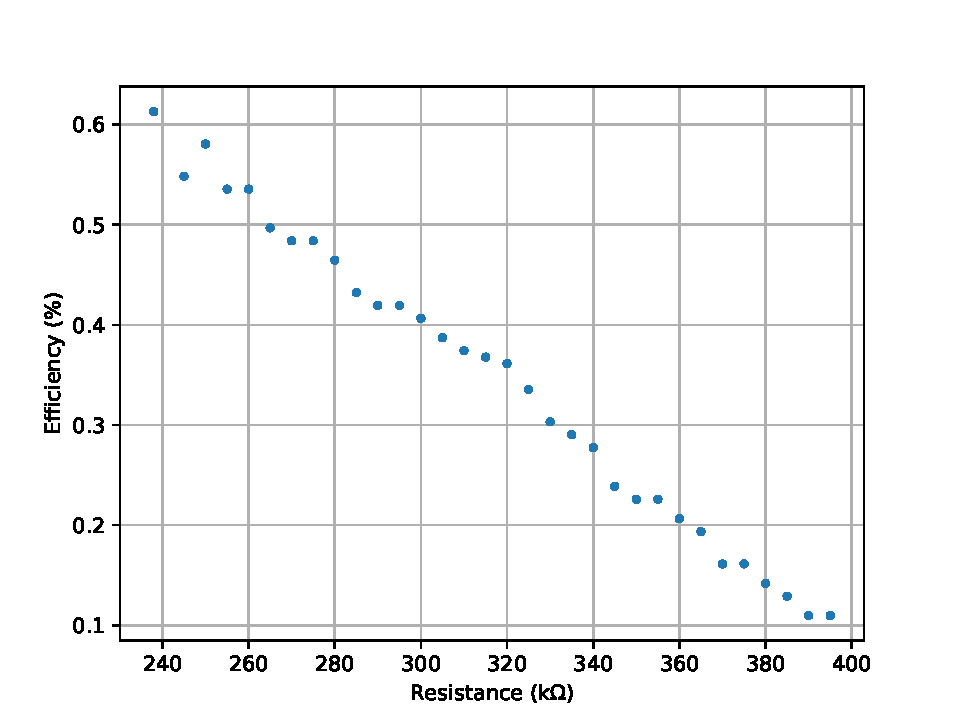
\includegraphics[width = .8\textwidth]{Images/efficiency.pdf}
  \caption{Efficiency of the doubling crystal versus the resistance of the thermistor (and thus temperature of the crystal) without realignment of the laser beam through the crystal. While it appears that the efficiency decreases with increasing temperature, the maximum efficiency of 65\% could always be restored through realignment, indicating that the decrease is caused by misalignment and not temperature dependence.}
  \label{fig:crystaleff}
\end{figure}
